\section{Allocazione}
L'allocazione del file su disco può avvenire in più modi.

\subsubsection{Allocazione Contigua}
Il file viene scritto in locazioni contigue di memoria, ha il vantaggio che è necessario solo un indirizzo iniziale e la lunghezza, ma spesso non è semplice conoscere la lunghezza a priori e si rischia di generare frammentazione.

I blocchi logici non devono essere uguali a quelli fisici, se ho blocchi fisici da 512 byte posso dividerlo in 10 blocchi logici da circa 51 byte, riducendo così la frammentazione. Con dei puntatori è possibile anche distribuire i file nel disco, senza che siano fisicamente contigui.

\begin{figure}[H]
    \centering
    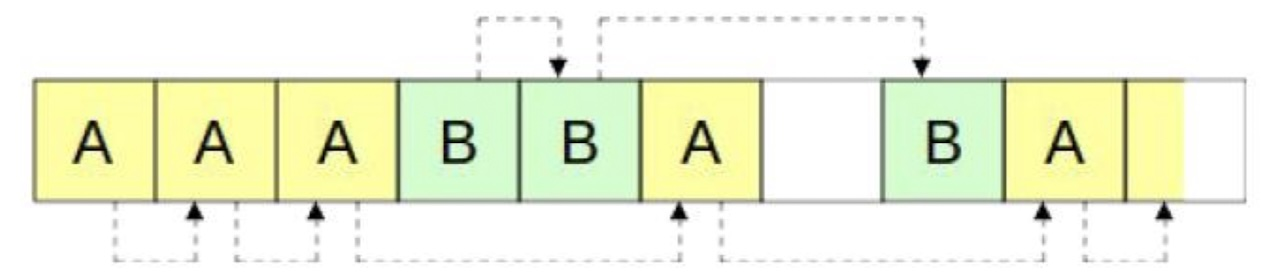
\includegraphics[width=0.4\linewidth]{assets/allocazione-contigua.jpeg}
\end{figure}

\subsubsection{Allocazione Concatenata}
Il file può essere sparso in tutto il disco, ogni blocco contiene un puntatore al blocco successivo.

\begin{figure}[H]
    \centering
    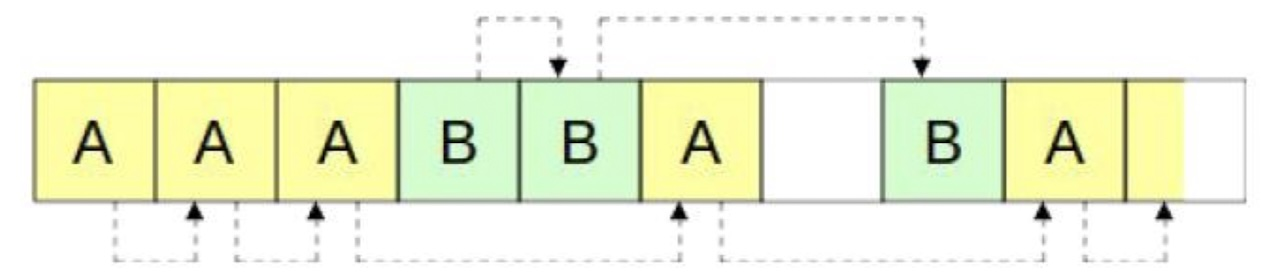
\includegraphics[width=0.4\linewidth]{assets/allocazione-contigua.jpeg}
\end{figure}


Esempio di questa tecnica è il file system FAT (File Allocation Table), sviluppato per MS-DOS.

Essa mantiene una tabella con un identificativo del file e l'indirizzo di inizio del file sul disco.

\spacer
La prima versione, FAT32 è limitata nella dimensione massima del disco, e dei file, a 4GB. exFAT elimina questa limitazione utilizzando indirizzi a 64 bit ed è supportata da tutti i sistemi operativi moderni.

Windows ora si è spostato su NTFS con piani per arrivare ad utilizzare ReFS  sempre più avanzati per soddisfare le richieste degli utenti.

\subsubsection{Allocazione Indicizzata}
Per ogni file si stabilisce un blocco indice, il quale contiene tutti i puntatori ai blocchi utilizzati dal file. Introduce quindi l'overhead per leggere il blocco indice, ma poi rimuove la frammentazione esterna del disco.

\begin{figure}[H]
    \centering
    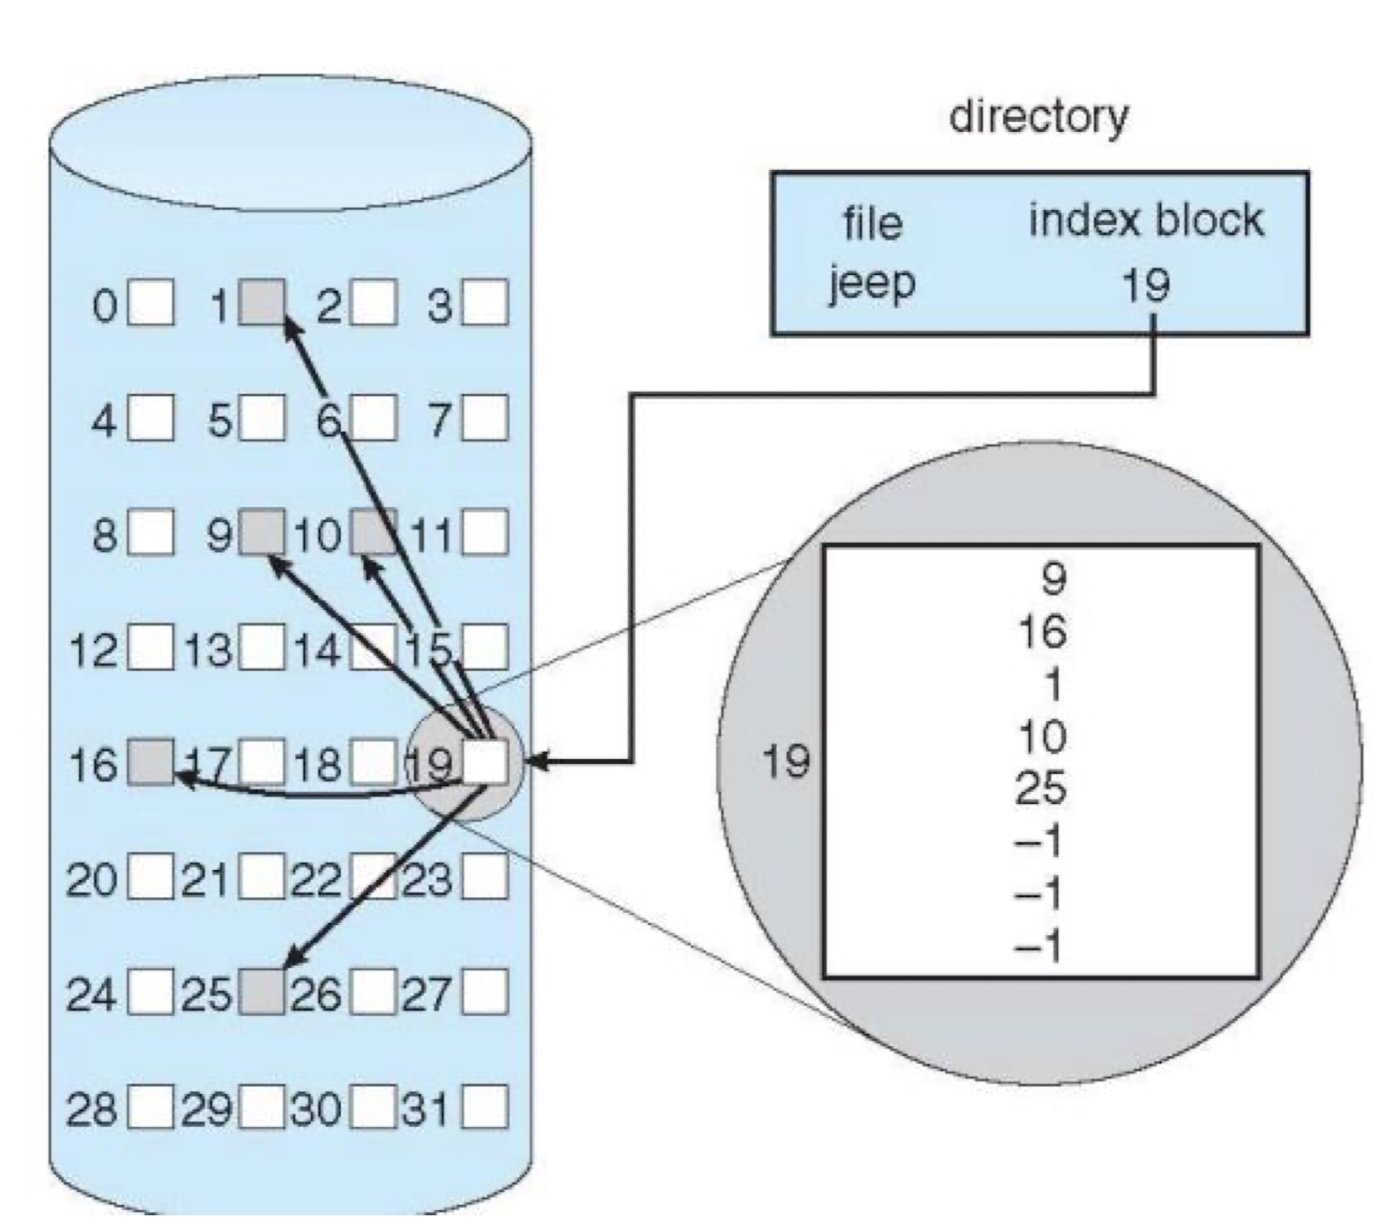
\includegraphics[width=0.5\linewidth]{assets/allocazione-indicizzata.jpg}
\end{figure}

Qualora i 512 puntatori non dovessero essere sufficienti si possono utilizzare delle tabelle concatenate con 511 puntatori a blocchi di memoria ciascuna.

\subsubsection{Mapping}
È possibile astrarre ulteriormente introducendo degli indirizzi logici dove il file risulta avere indirizzi contigui anche se gli indirizzi fisici non lo sono.

\spacer
Questo si può ottenere in più modi, tramite uno schema concatenato oppure tramite indici multilivello.

\spacer
Il primo, più semplice, prevede dei blocchi che puntano direttamene ai blocchi logici del file. Questi blocchi di indirizzi possono essere concatenati per ottenere una dimensione massima maggiore.

\begin{figure}[H]
    \centering
    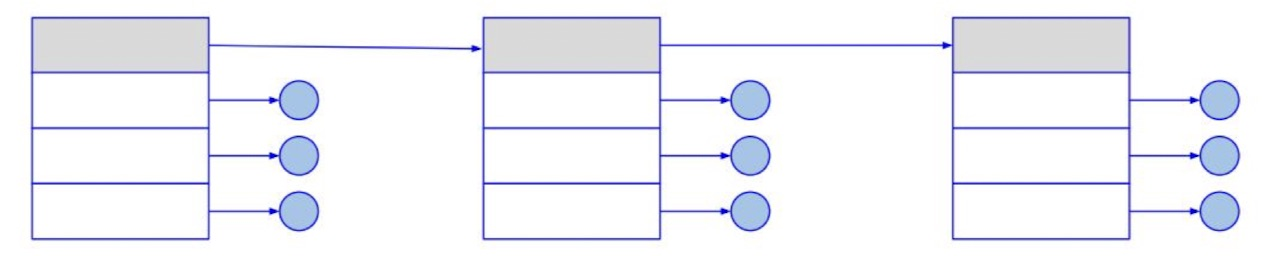
\includegraphics[width=0.5\linewidth]{assets/schema-concatenato.jpeg}
\end{figure}

\spacer
Il secondo utilizza più livelli per indicizzare una quantità maggiore di memoria.

\begin{figure}[H]
    \centering
    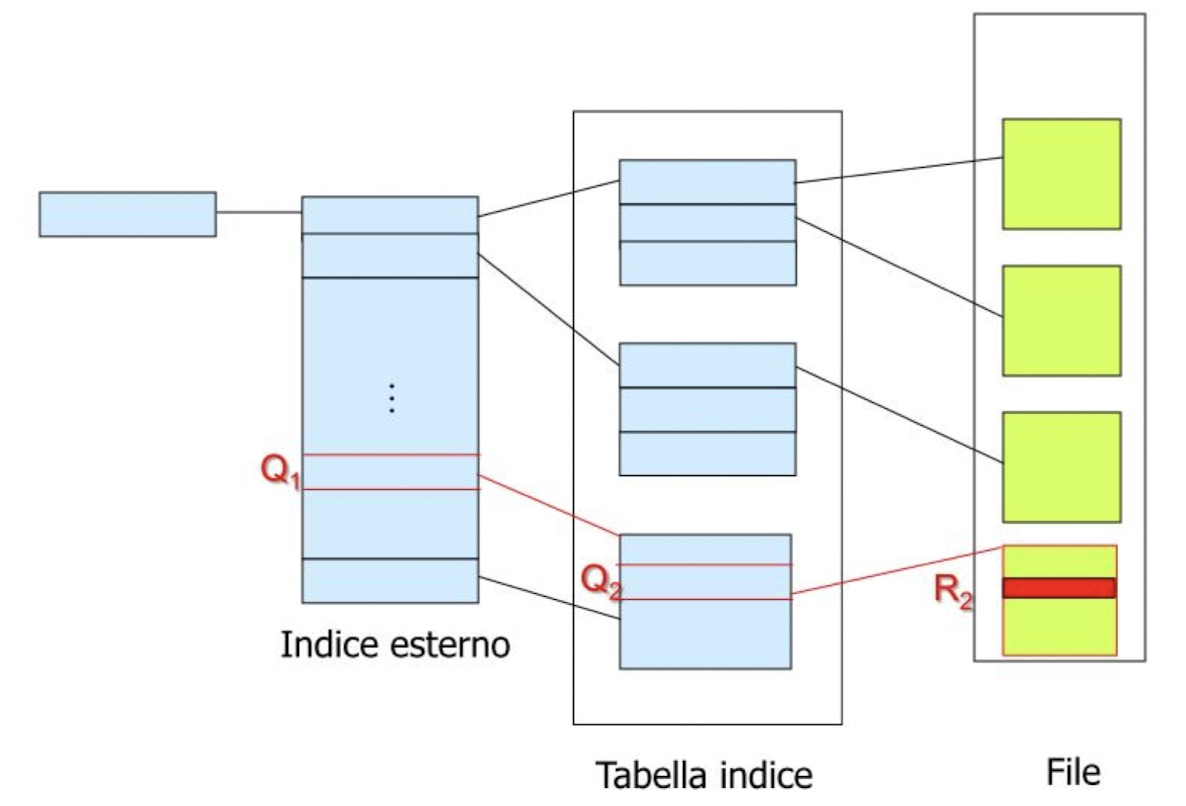
\includegraphics[width=0.4\linewidth]{assets/indici-multilivello.jpeg}
\end{figure}

\subsubsection{Schema Combinato}
Una soluzione ibrida viene spesso utilizzata nei sistemi operativi, ad esempio in unix, dove si mantiene un blocco per ogni file (inode) che contiene informazioni su di esso e un primo livello di indirizzi, alcuni sono diretti, altri sono multilivello a 2 o più livelli.

\begin{figure}[H]
    \centering
    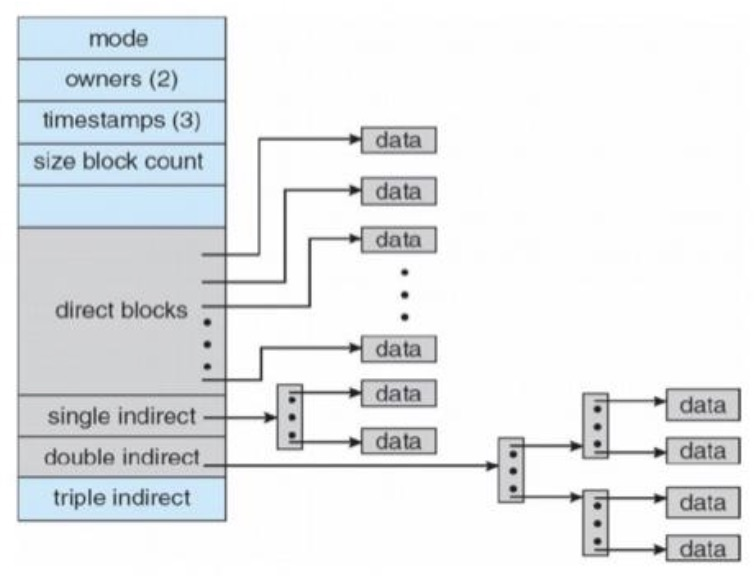
\includegraphics[width=0.4\linewidth]{assets/inode-ibrido.jpeg}
\end{figure}

\begin{sitemize}
    \item 0-10 indirizzi: inidirizzamento diretto
    \item 11° indirizzo: 1 livello
    \item 12° indirizzo: 2 livelli
    \item 13° indirizzo: 3 livelli
\end{sitemize}

\begin{note}
    In generale l'allocazione continua ha buone prestazioni sia per l'accesso casuale sia per quello sequenziale, l'allocazione concatenata è ottimale per l'accesso sequenziale.

    \spacer
    L'allocazione indicizzata è più complessa, un singolo accesso al disco può richiederne molti, è quindi importante gestire correttamente il clustering dei dati.
\end{note}

\subsection{Spazio Libero}
Per scegliere dove inserire i nuovi file è importante tenere traccia dello spazio libero nel disco.

Poi quando si crea un nuovo file si cercano blocchi liberi dalla struttura dati e quando si eliminano si raggiungono i blocchi nella struttura.

\subsubsection{Bitmap}
\begin{figure}[H]
    \centering
    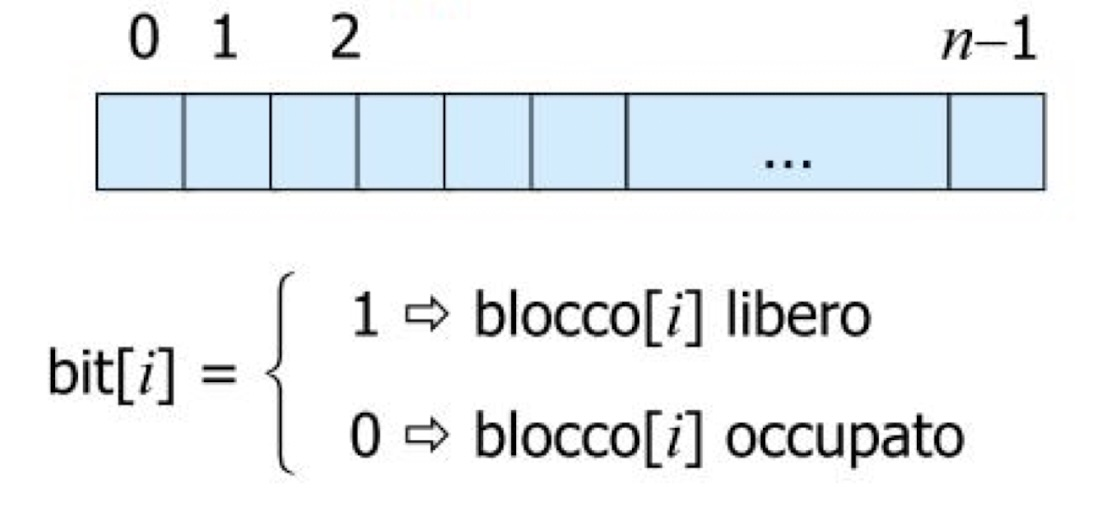
\includegraphics[width=0.4\linewidth]{assets/bitmap-libero.jpeg}
\end{figure}

È possibile mantenere un vettore dove ogni bit rappresenta un blocco, questa struttura dati ha buone prestazioni quando il vettore può essere mantenuto in memoria principale.

\subsubsection{Lista Concatenata}
Tutti i blocchi liberi si collegano mediante puntatori e si mantiene il puntatore della testa della lista in memoria centrale. È inefficiente per trovare spazi contigui di memoria.

\begin{figure}[H]
    \centering
    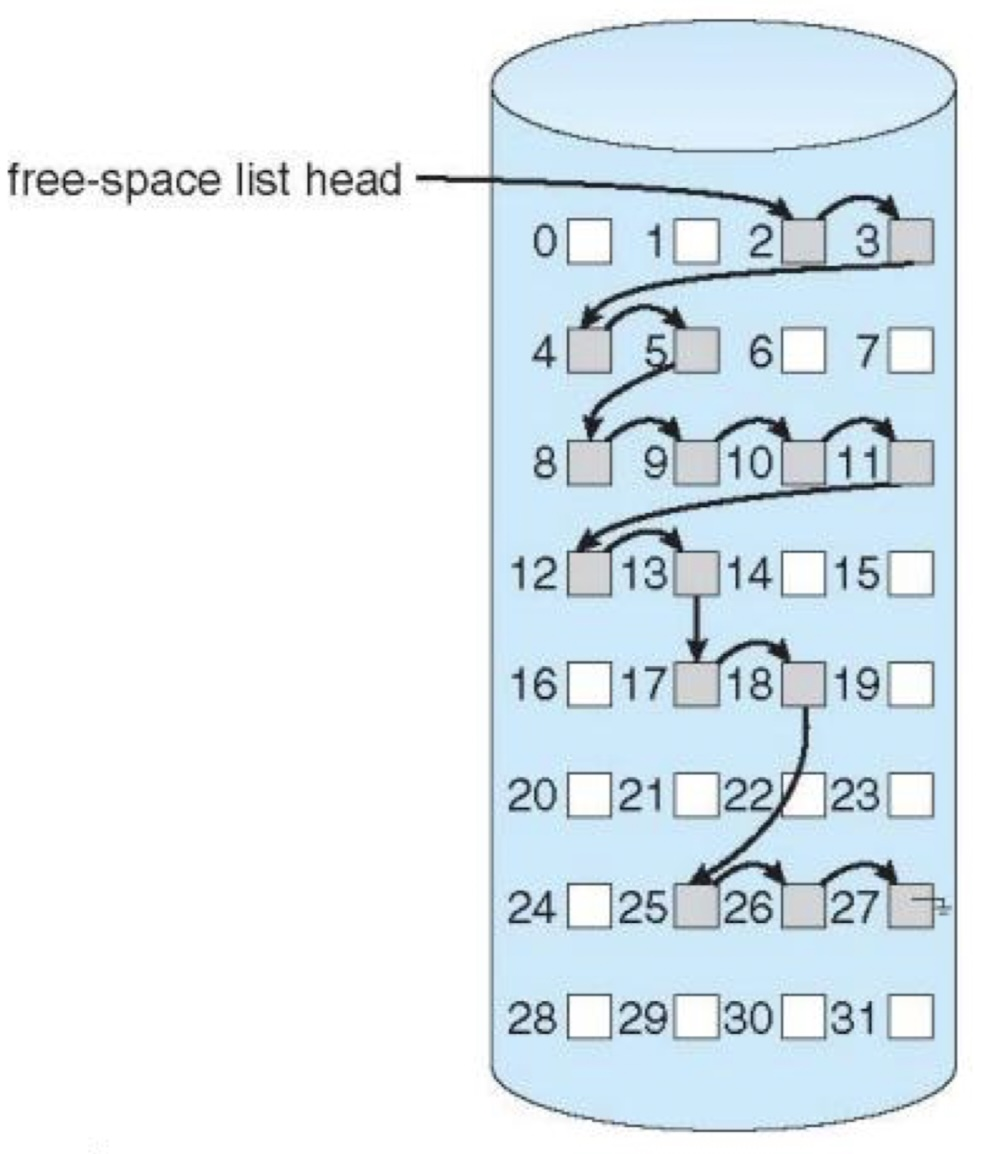
\includegraphics[width=0.3\linewidth]{assets/spazio-libero-lista-concatenata.jpg}
\end{figure}


\subsubsection{Grouping}
Creazione di $n$ blocchi, sul primo vengono salvati gli indirizzi dei blocchi liberi, che inizialmente sono $n-1$

\subsubsection{Conteggio}
Se lo spazio viene allocato e liberato in modo contiguo è possibile mantenere semplicemente un indirizzo sul disco e il numero di blocchi liberi contigui successivi all'indirizzo.

\begin{note}
    TRIM è un comando ATA che consente al Sistema Operativo di comunicare ai dischi quali blocchi di dati possono essere eliminati.

    Questo permette agli SSD di meglio gestire i dati, senza copiare file che verranno poi eliminati.
\end{note}

\subsection{Prestazioni}
Per ottimizzare le prestazioni i dati e metadati vengono mantenuti in locazioni di memoria vicine nel disco.
Anche le dimensioni dei puntatori vanno valutate attentamente, puntatori di dimensioni maggiori permettono di indicizzare una maggior quantità di memoria, ma richiedono più spazio di memorizzazione.

\spacer
Per le letture/scritture asincrone è possibile utilizzare delle cache, inizialmente si utilizzava una cache sul dispositivo ed una sulla memoria principale.

Da quando le cache sono aumentate di dimensione è possibile utilizzare solo quella del dispositivo.

\spacer
L'algoritmo di rimpiazzo LRU per questa cache non è efficiente (una volta letto un dato difficilmente viene letto nuovamente), si preferisce quindi un algoritmo free-behind (che rilascia la pagina più lontana dall'indirizzo corrente) oppure read-ahead (che carica sia la pagina richiesta che quelle successive)

\subsection{Incoerenze}
I file sono mantenuti parzialmente in memoria ram e nel disco, con un sistema di sincronizzazione non istantaneo, per questo motivo in caso di malfunzionamento del sistema si possono generare delle incoerenze che vanno correttamente gestite.

\spacer
Per risolvere questo problema si possono utilizzare dei programmi (es. \texttt{chkdsk} in UNIX) che confrontano i dati sul disco e quelli sulla directory alla ricerca di possibili incoerenze.

Inoltre è possibile effettuare dei backup dei dati del disco da cui recuperare file persi o danneggiati.

\subsection{Accesso al File}
Approfondiamo le strategie che possono essere utilizzate per accedere ai file, in particolare vediamo:

\begin{sitemize}
    \item \textbf{Accesso Sequenziale:} I dati vengono letti un blocco alla volta e il puntatore avanza ad ogni lettura o scrittura in modo regolare.

    \item \textbf{Accesso Diretto:} I dati vengono letti da posizioni arbitrarie senza dover rispettare un determinato ordine.

    \begin{figure}[H]
        \centering
        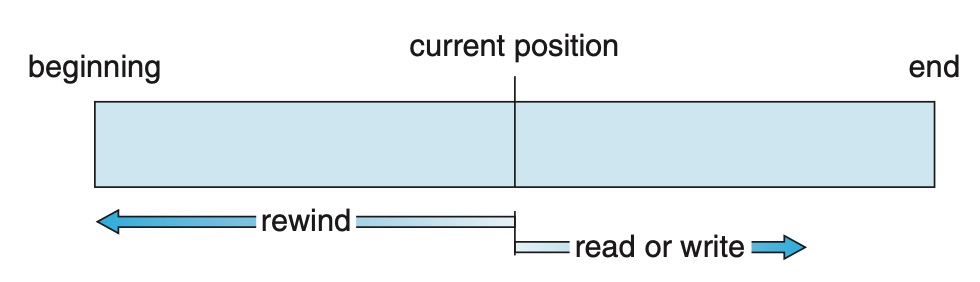
\includegraphics[width=0.5\linewidth]{assets/accesso-diretto.jpg}
    \end{figure}
    \item \textbf{Accesso Indicizzato:} Strategia costruita sull'accesso diretto, in aggiunta viene costruito un file di indice per l'accesso al file stesso.

    Il file contiene dei puntatori al file stesso, prima di accedere al file serve quindi fare una ricerca nell'indice.

    \begin{figure}[H]
        \centering
        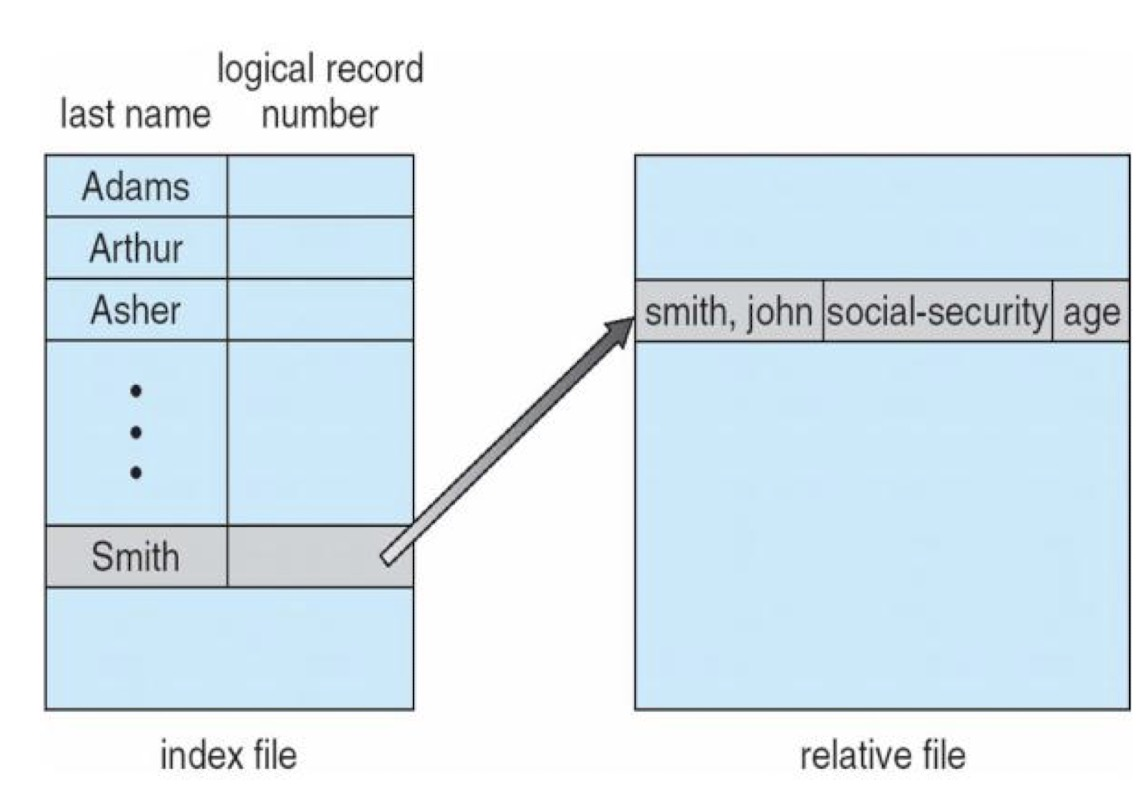
\includegraphics[width=0.4\linewidth]{assets/accesso-indicizzato.jpg}
    \end{figure}
\end{sitemize}
